\makeatletter
\newcommand*{\textoverline}[1]{$\overline{\hbox{#1}}\m@th$}
\makeatother

\subsection{Levelshifters}\label{sec:levelshifter}
To generate suffici\"{e} output power thick oxide transitors are used at the output stage. One of the problems with this is that these transistors have a much larger threshold voltage and that they operate at larger supply voltages than the low voltage transistors. Because of this the fast low voltage transitors used in the digital front end and for mixing cannot generate a large enough V\textsubscript{ON}. Raising the supply voltage to the low voltage transistors in order to increase the output voltage of the mixers will break them. So special care has to be taken when a transition from a low voltage circuit to high voltage thick oxide transistors. To this end a level shifter is designed. In this design special care will be taken to ensure that the voltages accros any low voltage transistor will not exceed 1.1V, so they will not break. On the output side is has to be able to drive relatively large transistors. Also in the on state it must supply a voltage of approximately 2V and in the offstate a voltage smaller than 0.7V. 
In~\cite{powerdac} a design for the levelshifter was proposed, but they were not able to integrate it with the rest of their design. However, they did show work that it worked in a standalone simulation. The main problem are difficulties with the cadence models of the thick oxide transistors used for simulation. These models show strange behavior and have an unrealistically high threshold voltage of 1.5V. Also a design proposed in~\cite{hass2000level} was considered. But due to the increased complexity combined with our models and its multiple stages, which are bad for timing performance, this design was not used. That design has an propagation delay of roughly 10 ns, which is not acceptable for this paper's design. 
\begin{figure}[h]
 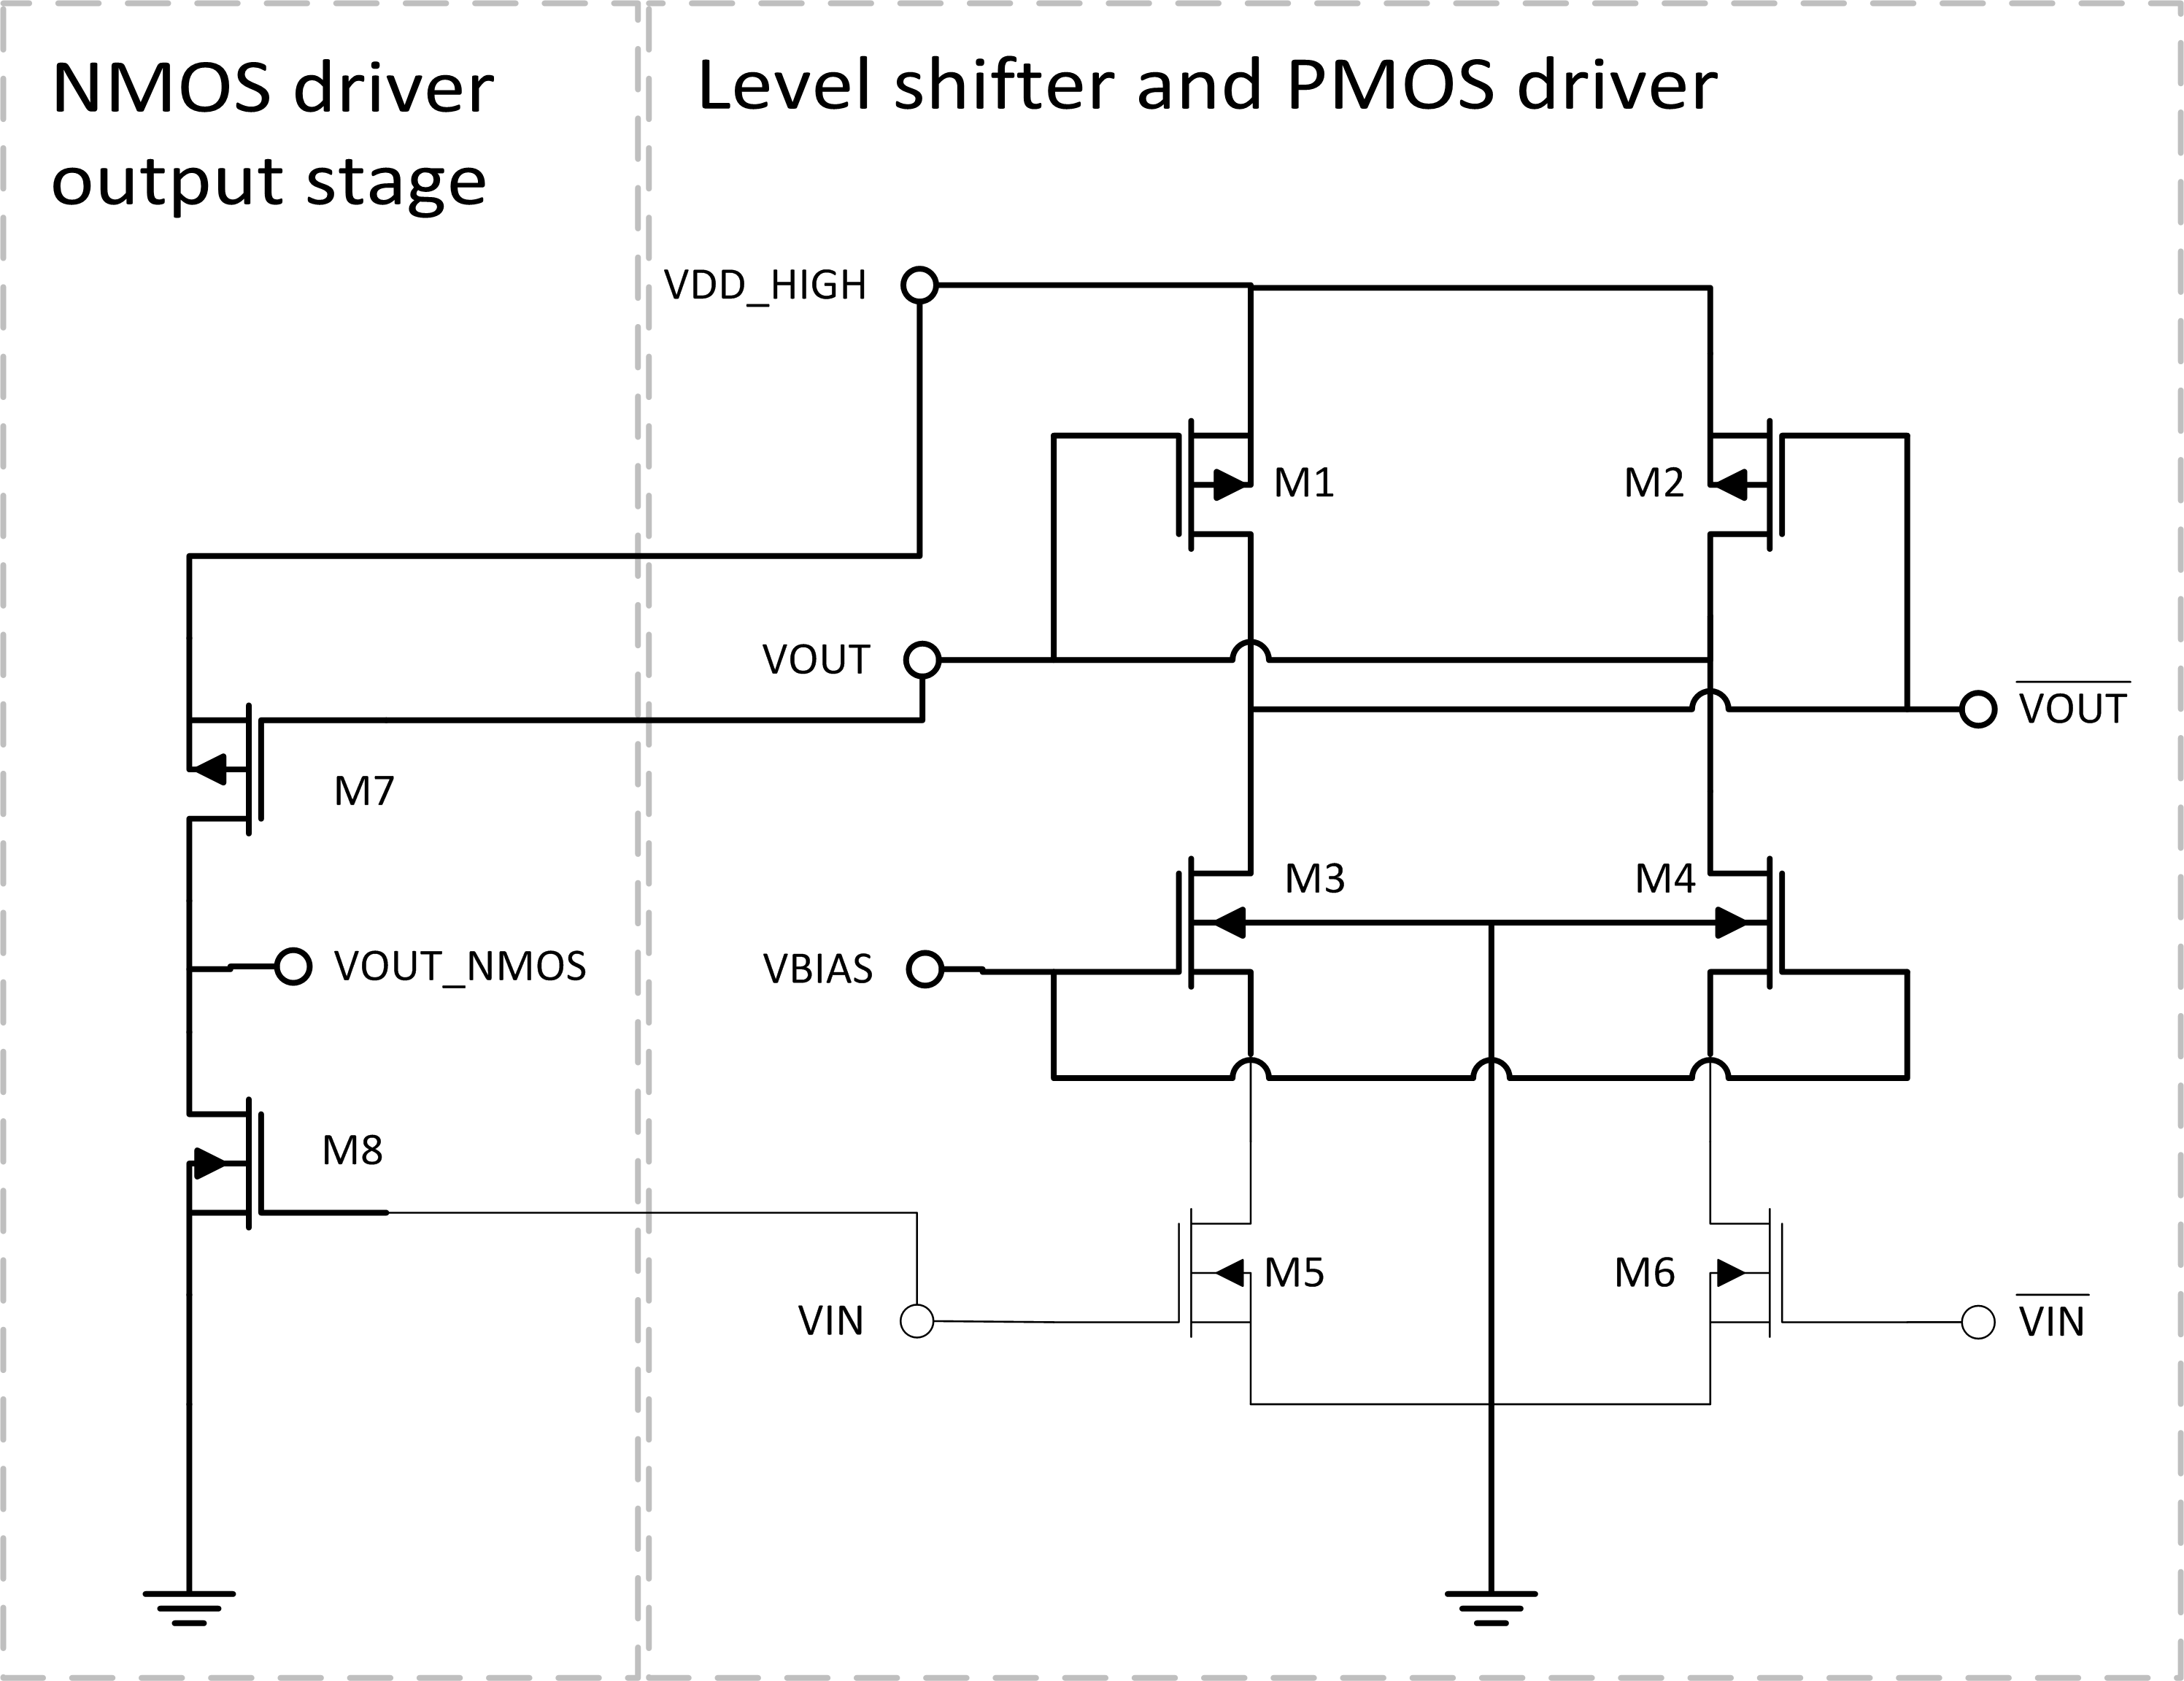
\includegraphics[width=0.5\textwidth]{levelshifter_schematic}
 \caption{Schematics of the levelshifter, thick wires indicate a high voltage regime and thing the low voltage transistors}
 \label{fig:schematic_levelshifter}
\end{figure}
The chosen design is a modified version of the one proposed in~\cite{powerdac} and is shown in Fig.~\ref{fig:schematic_levelshifter}. The inputs are connected to the gates of the low voltage transistors M5 and M6 and have an input range of 0V(off) to 1.1V(on). For correct operation VIN and \textoverline{VIN} must be each other's logical inverse. VBIAS is set to ??V and is connected to the gates of M3 and M4. These transistors protect M5 and M6 from the high supply voltage. M1 and M2 provide an positive feed back loop, which makes the circuit function. Its operation is explained using a low to high transition, so initially VIN is 0V, \textoverline{VIN} is 1.1V, VOUT is on its off value and \textoverline{VOUT} is 2V. In this situation only the right branch is conducting current, because \textoverline{VIN} is high and since there is no current in the left branch \textoverline{VOUT} is low. When VIN transitions to a high state, it starts conducting current, forcing VM5 to go a bit higher, as well as \textoverline{VOUT}. Because \textoverline{VOUT} increases, the current through the right branch decreases as well as VOUT. The decreased VOUT makes the left branch conduct more current and \textoverline{VOUT} go higher. Due to this postive feedback loop VOUT will go to VDD.